% Options for packages loaded elsewhere
% Options for packages loaded elsewhere
\PassOptionsToPackage{unicode}{hyperref}
\PassOptionsToPackage{hyphens}{url}
\PassOptionsToPackage{dvipsnames,svgnames,x11names}{xcolor}
%
\documentclass[
  spanish,
  letterpaper,
  DIV=11,
  numbers=noendperiod]{scrreprt}
\usepackage{xcolor}
\usepackage{amsmath,amssymb}
\setcounter{secnumdepth}{5}
\usepackage{iftex}
\ifPDFTeX
  \usepackage[T1]{fontenc}
  \usepackage[utf8]{inputenc}
  \usepackage{textcomp} % provide euro and other symbols
\else % if luatex or xetex
  \usepackage{unicode-math} % this also loads fontspec
  \defaultfontfeatures{Scale=MatchLowercase}
  \defaultfontfeatures[\rmfamily]{Ligatures=TeX,Scale=1}
\fi
\usepackage{lmodern}
\ifPDFTeX\else
  % xetex/luatex font selection
\fi
% Use upquote if available, for straight quotes in verbatim environments
\IfFileExists{upquote.sty}{\usepackage{upquote}}{}
\IfFileExists{microtype.sty}{% use microtype if available
  \usepackage[]{microtype}
  \UseMicrotypeSet[protrusion]{basicmath} % disable protrusion for tt fonts
}{}
\makeatletter
\@ifundefined{KOMAClassName}{% if non-KOMA class
  \IfFileExists{parskip.sty}{%
    \usepackage{parskip}
  }{% else
    \setlength{\parindent}{0pt}
    \setlength{\parskip}{6pt plus 2pt minus 1pt}}
}{% if KOMA class
  \KOMAoptions{parskip=half}}
\makeatother
% Make \paragraph and \subparagraph free-standing
\makeatletter
\ifx\paragraph\undefined\else
  \let\oldparagraph\paragraph
  \renewcommand{\paragraph}{
    \@ifstar
      \xxxParagraphStar
      \xxxParagraphNoStar
  }
  \newcommand{\xxxParagraphStar}[1]{\oldparagraph*{#1}\mbox{}}
  \newcommand{\xxxParagraphNoStar}[1]{\oldparagraph{#1}\mbox{}}
\fi
\ifx\subparagraph\undefined\else
  \let\oldsubparagraph\subparagraph
  \renewcommand{\subparagraph}{
    \@ifstar
      \xxxSubParagraphStar
      \xxxSubParagraphNoStar
  }
  \newcommand{\xxxSubParagraphStar}[1]{\oldsubparagraph*{#1}\mbox{}}
  \newcommand{\xxxSubParagraphNoStar}[1]{\oldsubparagraph{#1}\mbox{}}
\fi
\makeatother

\usepackage{color}
\usepackage{fancyvrb}
\newcommand{\VerbBar}{|}
\newcommand{\VERB}{\Verb[commandchars=\\\{\}]}
\DefineVerbatimEnvironment{Highlighting}{Verbatim}{commandchars=\\\{\}}
% Add ',fontsize=\small' for more characters per line
\usepackage{framed}
\definecolor{shadecolor}{RGB}{241,243,245}
\newenvironment{Shaded}{\begin{snugshade}}{\end{snugshade}}
\newcommand{\AlertTok}[1]{\textcolor[rgb]{0.68,0.00,0.00}{#1}}
\newcommand{\AnnotationTok}[1]{\textcolor[rgb]{0.37,0.37,0.37}{#1}}
\newcommand{\AttributeTok}[1]{\textcolor[rgb]{0.40,0.45,0.13}{#1}}
\newcommand{\BaseNTok}[1]{\textcolor[rgb]{0.68,0.00,0.00}{#1}}
\newcommand{\BuiltInTok}[1]{\textcolor[rgb]{0.00,0.23,0.31}{#1}}
\newcommand{\CharTok}[1]{\textcolor[rgb]{0.13,0.47,0.30}{#1}}
\newcommand{\CommentTok}[1]{\textcolor[rgb]{0.37,0.37,0.37}{#1}}
\newcommand{\CommentVarTok}[1]{\textcolor[rgb]{0.37,0.37,0.37}{\textit{#1}}}
\newcommand{\ConstantTok}[1]{\textcolor[rgb]{0.56,0.35,0.01}{#1}}
\newcommand{\ControlFlowTok}[1]{\textcolor[rgb]{0.00,0.23,0.31}{\textbf{#1}}}
\newcommand{\DataTypeTok}[1]{\textcolor[rgb]{0.68,0.00,0.00}{#1}}
\newcommand{\DecValTok}[1]{\textcolor[rgb]{0.68,0.00,0.00}{#1}}
\newcommand{\DocumentationTok}[1]{\textcolor[rgb]{0.37,0.37,0.37}{\textit{#1}}}
\newcommand{\ErrorTok}[1]{\textcolor[rgb]{0.68,0.00,0.00}{#1}}
\newcommand{\ExtensionTok}[1]{\textcolor[rgb]{0.00,0.23,0.31}{#1}}
\newcommand{\FloatTok}[1]{\textcolor[rgb]{0.68,0.00,0.00}{#1}}
\newcommand{\FunctionTok}[1]{\textcolor[rgb]{0.28,0.35,0.67}{#1}}
\newcommand{\ImportTok}[1]{\textcolor[rgb]{0.00,0.46,0.62}{#1}}
\newcommand{\InformationTok}[1]{\textcolor[rgb]{0.37,0.37,0.37}{#1}}
\newcommand{\KeywordTok}[1]{\textcolor[rgb]{0.00,0.23,0.31}{\textbf{#1}}}
\newcommand{\NormalTok}[1]{\textcolor[rgb]{0.00,0.23,0.31}{#1}}
\newcommand{\OperatorTok}[1]{\textcolor[rgb]{0.37,0.37,0.37}{#1}}
\newcommand{\OtherTok}[1]{\textcolor[rgb]{0.00,0.23,0.31}{#1}}
\newcommand{\PreprocessorTok}[1]{\textcolor[rgb]{0.68,0.00,0.00}{#1}}
\newcommand{\RegionMarkerTok}[1]{\textcolor[rgb]{0.00,0.23,0.31}{#1}}
\newcommand{\SpecialCharTok}[1]{\textcolor[rgb]{0.37,0.37,0.37}{#1}}
\newcommand{\SpecialStringTok}[1]{\textcolor[rgb]{0.13,0.47,0.30}{#1}}
\newcommand{\StringTok}[1]{\textcolor[rgb]{0.13,0.47,0.30}{#1}}
\newcommand{\VariableTok}[1]{\textcolor[rgb]{0.07,0.07,0.07}{#1}}
\newcommand{\VerbatimStringTok}[1]{\textcolor[rgb]{0.13,0.47,0.30}{#1}}
\newcommand{\WarningTok}[1]{\textcolor[rgb]{0.37,0.37,0.37}{\textit{#1}}}

\usepackage{longtable,booktabs,array}
\usepackage{calc} % for calculating minipage widths
% Correct order of tables after \paragraph or \subparagraph
\usepackage{etoolbox}
\makeatletter
\patchcmd\longtable{\par}{\if@noskipsec\mbox{}\fi\par}{}{}
\makeatother
% Allow footnotes in longtable head/foot
\IfFileExists{footnotehyper.sty}{\usepackage{footnotehyper}}{\usepackage{footnote}}
\makesavenoteenv{longtable}
\usepackage{graphicx}
\makeatletter
\newsavebox\pandoc@box
\newcommand*\pandocbounded[1]{% scales image to fit in text height/width
  \sbox\pandoc@box{#1}%
  \Gscale@div\@tempa{\textheight}{\dimexpr\ht\pandoc@box+\dp\pandoc@box\relax}%
  \Gscale@div\@tempb{\linewidth}{\wd\pandoc@box}%
  \ifdim\@tempb\p@<\@tempa\p@\let\@tempa\@tempb\fi% select the smaller of both
  \ifdim\@tempa\p@<\p@\scalebox{\@tempa}{\usebox\pandoc@box}%
  \else\usebox{\pandoc@box}%
  \fi%
}
% Set default figure placement to htbp
\def\fps@figure{htbp}
\makeatother



\ifLuaTeX
\usepackage[bidi=basic]{babel}
\else
\usepackage[bidi=default]{babel}
\fi
% get rid of language-specific shorthands (see #6817):
\let\LanguageShortHands\languageshorthands
\def\languageshorthands#1{}


\setlength{\emergencystretch}{3em} % prevent overfull lines

\providecommand{\tightlist}{%
  \setlength{\itemsep}{0pt}\setlength{\parskip}{0pt}}



 


\KOMAoption{captions}{tableheading}
\makeatletter
\@ifpackageloaded{tcolorbox}{}{\usepackage[skins,breakable]{tcolorbox}}
\@ifpackageloaded{fontawesome5}{}{\usepackage{fontawesome5}}
\definecolor{quarto-callout-color}{HTML}{909090}
\definecolor{quarto-callout-note-color}{HTML}{0758E5}
\definecolor{quarto-callout-important-color}{HTML}{CC1914}
\definecolor{quarto-callout-warning-color}{HTML}{EB9113}
\definecolor{quarto-callout-tip-color}{HTML}{00A047}
\definecolor{quarto-callout-caution-color}{HTML}{FC5300}
\definecolor{quarto-callout-color-frame}{HTML}{acacac}
\definecolor{quarto-callout-note-color-frame}{HTML}{4582ec}
\definecolor{quarto-callout-important-color-frame}{HTML}{d9534f}
\definecolor{quarto-callout-warning-color-frame}{HTML}{f0ad4e}
\definecolor{quarto-callout-tip-color-frame}{HTML}{02b875}
\definecolor{quarto-callout-caution-color-frame}{HTML}{fd7e14}
\makeatother
\makeatletter
\@ifpackageloaded{bookmark}{}{\usepackage{bookmark}}
\makeatother
\makeatletter
\@ifpackageloaded{caption}{}{\usepackage{caption}}
\AtBeginDocument{%
\ifdefined\contentsname
  \renewcommand*\contentsname{Tabla de contenidos}
\else
  \newcommand\contentsname{Tabla de contenidos}
\fi
\ifdefined\listfigurename
  \renewcommand*\listfigurename{Listado de Figuras}
\else
  \newcommand\listfigurename{Listado de Figuras}
\fi
\ifdefined\listtablename
  \renewcommand*\listtablename{Listado de Tablas}
\else
  \newcommand\listtablename{Listado de Tablas}
\fi
\ifdefined\figurename
  \renewcommand*\figurename{Figura}
\else
  \newcommand\figurename{Figura}
\fi
\ifdefined\tablename
  \renewcommand*\tablename{Tabla}
\else
  \newcommand\tablename{Tabla}
\fi
}
\@ifpackageloaded{float}{}{\usepackage{float}}
\floatstyle{ruled}
\@ifundefined{c@chapter}{\newfloat{codelisting}{h}{lop}}{\newfloat{codelisting}{h}{lop}[chapter]}
\floatname{codelisting}{Listado}
\newcommand*\listoflistings{\listof{codelisting}{Listado de Listados}}
\makeatother
\makeatletter
\makeatother
\makeatletter
\@ifpackageloaded{caption}{}{\usepackage{caption}}
\@ifpackageloaded{subcaption}{}{\usepackage{subcaption}}
\makeatother
\usepackage{bookmark}
\IfFileExists{xurl.sty}{\usepackage{xurl}}{} % add URL line breaks if available
\urlstyle{same}
\hypersetup{
  pdftitle={Notas de clase Business Analytics},
  pdfauthor={Daniel Parra},
  pdflang={es},
  colorlinks=true,
  linkcolor={blue},
  filecolor={Maroon},
  citecolor={Blue},
  urlcolor={Blue},
  pdfcreator={LaTeX via pandoc}}


\title{Notas de clase Business Analytics}
\author{Daniel Parra}
\date{Invalid Date}
\begin{document}
\maketitle

\renewcommand*\contentsname{Tabla de contenidos}
{
\hypersetup{linkcolor=}
\setcounter{tocdepth}{2}
\tableofcontents
}

\bookmarksetup{startatroot}

\chapter*{Bienvenidos}\label{bienvenidos}
\addcontentsline{toc}{chapter}{Bienvenidos}

\markboth{Bienvenidos}{Bienvenidos}

Este libro ha sido creado con el propósito de ofrecer un resumen claro y
conciso de los conceptos clave de las clases de Business Analytics para
los posgrados de administración de la Pontificia Universidad Javeriana.
Es un complemento diseñado para reforzar el aprendizaje en clase, pero
no pretende reemplazar la experiencia educativa que estas ofrecen.

Parte del texto en estas notas de clase ha sido elaborado con ayuda de
inteligencia artificial (ChatGPT), combinando apuntes propios y
referencias de diversos libros. Las ilustraciones, inspiradas en el
libro ``Math with Bad Drawings'' de Ben Orlin, también han sido
generadas utilizando inteligencia artificial.

© 2025 Pontificia Universidad Javeriana. Este libro está licenciado bajo
una licencia CC BY 4.0.

\bookmarksetup{startatroot}

\chapter{Introducción: Descubriendo la Analítica de
Datos}\label{introducciuxf3n-descubriendo-la-analuxedtica-de-datos}

Imagina que trabajas en una empresa que debe decidir qué producto lanzar
o qué precio poner a sus artículos. ¿Cómo tomas estas decisiones?
Antiguamente, las decisiones se tomaban según la intuición del jefe
(\textbf{HiPPO}, la persona mejor pagada en la organización), pero
actualmente contamos con algo mejor: la analítica de datos.

\section{¿Qué es la Analítica de Datos para
Negocios?}\label{quuxe9-es-la-analuxedtica-de-datos-para-negocios}

La analítica de datos es la aplicación de herramientas tecnológicas y
estadísticas para analizar información relevante y apoyar la toma de
decisiones en una organización.

Los datos, sin embargo, no son suficientes por sí solos. Necesitamos
interpretarlos de manera efectiva para contar historias convincentes que
permitan tomar decisiones informadas.

\section{¿Qué tipo de preguntas podemos responder con la
analítica?}\label{quuxe9-tipo-de-preguntas-podemos-responder-con-la-analuxedtica}

La analítica de negocios nos permite responder preguntas prácticas,
como:

\begin{itemize}
\tightlist
\item
  ¿Quiénes son mis clientes?
\item
  ¿Qué campaña de marketing es más efectiva?
\item
  ¿Cuál sería el efecto de cambiar los precios?
\item
  ¿Cómo predecir la demanda de un producto?
\end{itemize}

\section{Tipos de Analítica}\label{tipos-de-analuxedtica}

Hay tres tipos principales de analítica:

\subsection{Analítica Descriptiva}\label{analuxedtica-descriptiva}

Describe la situación actual mediante visualizaciones y estadísticas
básicas.

\textbf{Ejemplos:}

\begin{itemize}
\tightlist
\item
  ¿Han crecido las ventas este año?
\item
  ¿Qué región vende menos?
\end{itemize}

\subsection{Analítica Predictiva}\label{analuxedtica-predictiva}

Predice qué sucederá, aprovechando correlaciones entre variables. Aquí
no es necesaria la causalidad, sino una relación estadística sólida.

\textbf{Ejemplos:}

\begin{itemize}
\tightlist
\item
  ¿Cuál es la probabilidad de que un cliente deje de comprar?
\item
  ¿Qué tan probable es que una transacción sea fraudulenta?
\end{itemize}

\subsection{Analítica Prescriptiva}\label{analuxedtica-prescriptiva}

Sugiere decisiones óptimas, enfocándose en relaciones causales y,
frecuentemente, utilizando experimentos.

\textbf{Ejemplos:}

\begin{itemize}
\tightlist
\item
  ¿Subir el precio incrementará las ganancias?
\item
  ¿Qué diseño de página web aumentará las ventas?
\end{itemize}

\section{La cadena de valor en Business
Analytics}\label{la-cadena-de-valor-en-business-analytics}

La analítica de negocios incluye:

\begin{itemize}
\tightlist
\item
  \textbf{Recolección y organización de datos:} Crear bases de datos
  (SQL, Power BI).
\item
  \textbf{Análisis de datos:} Usar herramientas como R, Excel o Python
  para análisis estratégicos.
\item
  \textbf{Comunicación de resultados:} Presentar hallazgos en reportes y
  visualizaciones (PowerPoint, Tableau, Quarto).
\end{itemize}

\bookmarksetup{startatroot}

\chapter{Capítulo 2}\label{capuxedtulo-2}

\section{Introducción}\label{introducciuxf3n}

Este es el nuevo capítulo 2.

\section{Contenido}\label{contenido}

Contenido del capítulo\ldots{}

\bookmarksetup{startatroot}

\chapter{Explorando tus Datos con Estadísticos
Descriptivos}\label{explorando-tus-datos-con-estaduxedsticos-descriptivos}

Imagina que eres gerente de un restaurante que acaba de lanzar un nuevo
menú y quieres evaluar la satisfacción de tus clientes a partir de las
calificaciones que te han dado. Tienes cientos de puntuaciones y
necesitas entender rápidamente cuál es la opinión general, qué tan
variadas son las experiencias y si hay patrones o valores atípicos que
merecen atención.

¿Cómo puedes resumir y comprender toda esa información de forma clara y
sencilla? Para eso utilizamos los estadísticos descriptivos,
herramientas fundamentales que nos permiten condensar grandes cantidades
de datos en medidas simples y significativas.

Estas medidas serán esenciales para tomar decisiones informadas que
mejoren tu decisiones.

\section{Estadísticos Descriptivos}\label{estaduxedsticos-descriptivos}

Los estadísticos descriptivos son herramientas clave que nos permiten
resumir y comprender mejor la información contenida en nuestros datos.
Para facilitar su estudio, los podemos clasificar en cuatro categorías
principales:

\begin{itemize}
\tightlist
\item
  \textbf{Medidas de tendencia central}: Estas nos muestran el valor
  típico o representativo en un conjunto de datos, es decir, alrededor
  de qué número se agrupan la mayoría de las observaciones.
\item
  \textbf{Medidas de variación}: Nos indican qué tan dispersos o
  concentrados están los datos respecto a esa tendencia central,
  ayudándonos a entender la consistencia o diversidad dentro de la
  información.
\item
  \textbf{Medidas de forma}: Describen la distribución general de los
  datos, revelando si están simétricos, sesgados hacia un lado o
  presentan picos o colas particulares.
\item
  \textbf{Medidas de relación}: Evalúan cómo dos variables numéricas se
  relacionan entre sí, especialmente si existe una conexión lineal que
  pueda ser útil para análisis más avanzados.
\end{itemize}

\section{Medidas de Tendencia
Central}\label{medidas-de-tendencia-central}

Cuando queremos entender las calificaciones que los clientes dan a tu
restaurante, buscamos encontrar un valor que represente lo que la
mayoría piensa. Las medidas de tendencia central nos ayudan a esto.

\subsection{Media (Promedio)}\label{media-promedio}

La media o promedio es una forma simple pero útil de resumir un conjunto
de datos. La media es el valor que obtienes al sumar todas las
calificaciones y dividirlas entre el número total de clientes.

\begin{tcolorbox}[enhanced jigsaw, bottomrule=.15mm, colframe=quarto-callout-tip-color-frame, breakable, colback=white, leftrule=.75mm, left=2mm, arc=.35mm, toprule=.15mm, opacityback=0, rightrule=.15mm]
\begin{minipage}[t]{5.5mm}
\textcolor{quarto-callout-tip-color}{\faLightbulb}
\end{minipage}%
\begin{minipage}[t]{\textwidth - 5.5mm}

Matemáticamente se escribiría así:

\[
\text{Media} = \bar{x} = \frac{x_1 + x_2 + \cdots + x_n}{n}
\]

\end{minipage}%
\end{tcolorbox}

Por ejemplo, si cinco clientes dieron las calificaciones: 4, 5, 3, 4 y
5, la media será:

\begin{tcolorbox}[enhanced jigsaw, bottomrule=.15mm, colframe=quarto-callout-tip-color-frame, breakable, colback=white, leftrule=.75mm, left=2mm, arc=.35mm, toprule=.15mm, opacityback=0, rightrule=.15mm]
\begin{minipage}[t]{5.5mm}
\textcolor{quarto-callout-tip-color}{\faLightbulb}
\end{minipage}%
\begin{minipage}[t]{\textwidth - 5.5mm}

\[
\bar{x} = \frac{4 + 5 + 3 + 4 + 5}{5} = \frac{21}{5} = 4.2
\]

\end{minipage}%
\end{tcolorbox}

Sin embargo la media, tiene limitaciones: no muestra cómo están
distribuidos los datos y puede ser engañosa si hay grandes diferencias
entre los valores. Por ejemplo:

\begin{center}
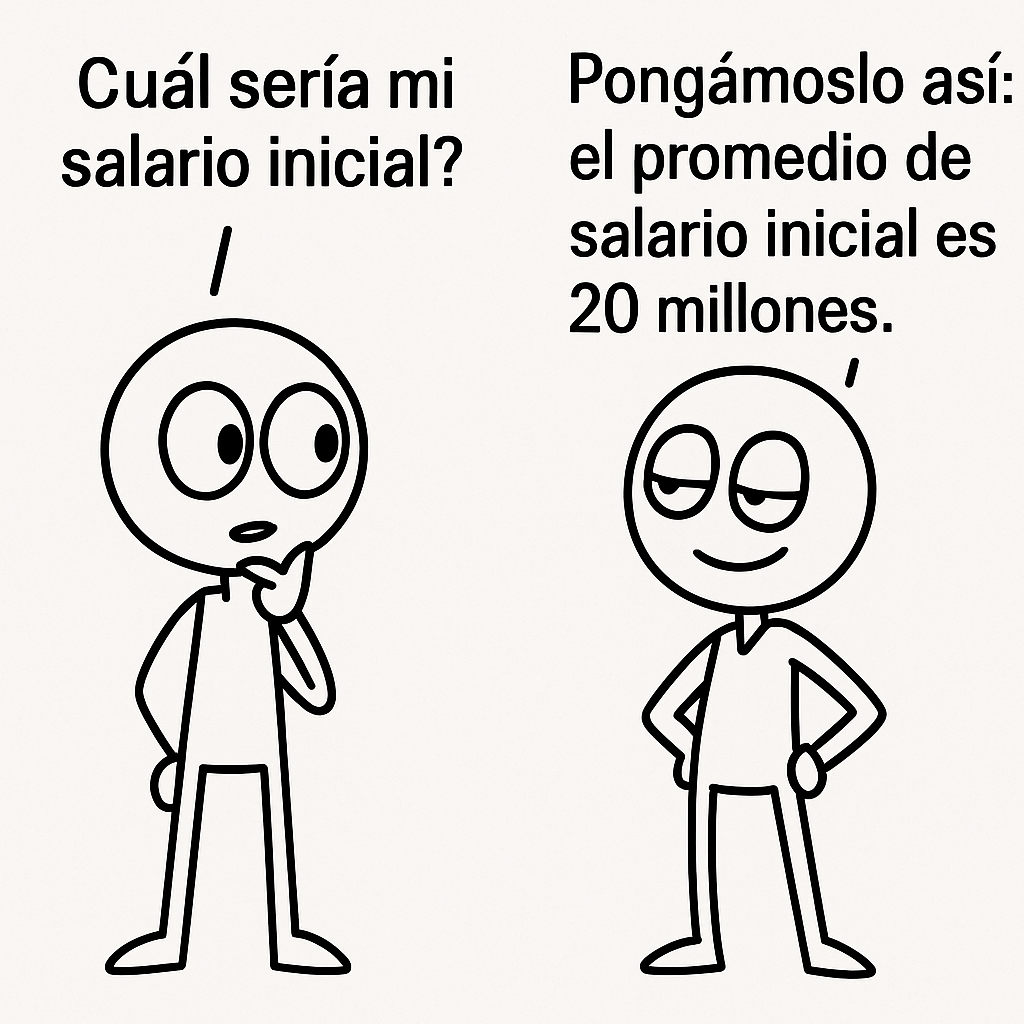
\includegraphics[width=3.64583in,height=\textheight,keepaspectratio]{img/media_1.png}
\end{center}

\begin{center}
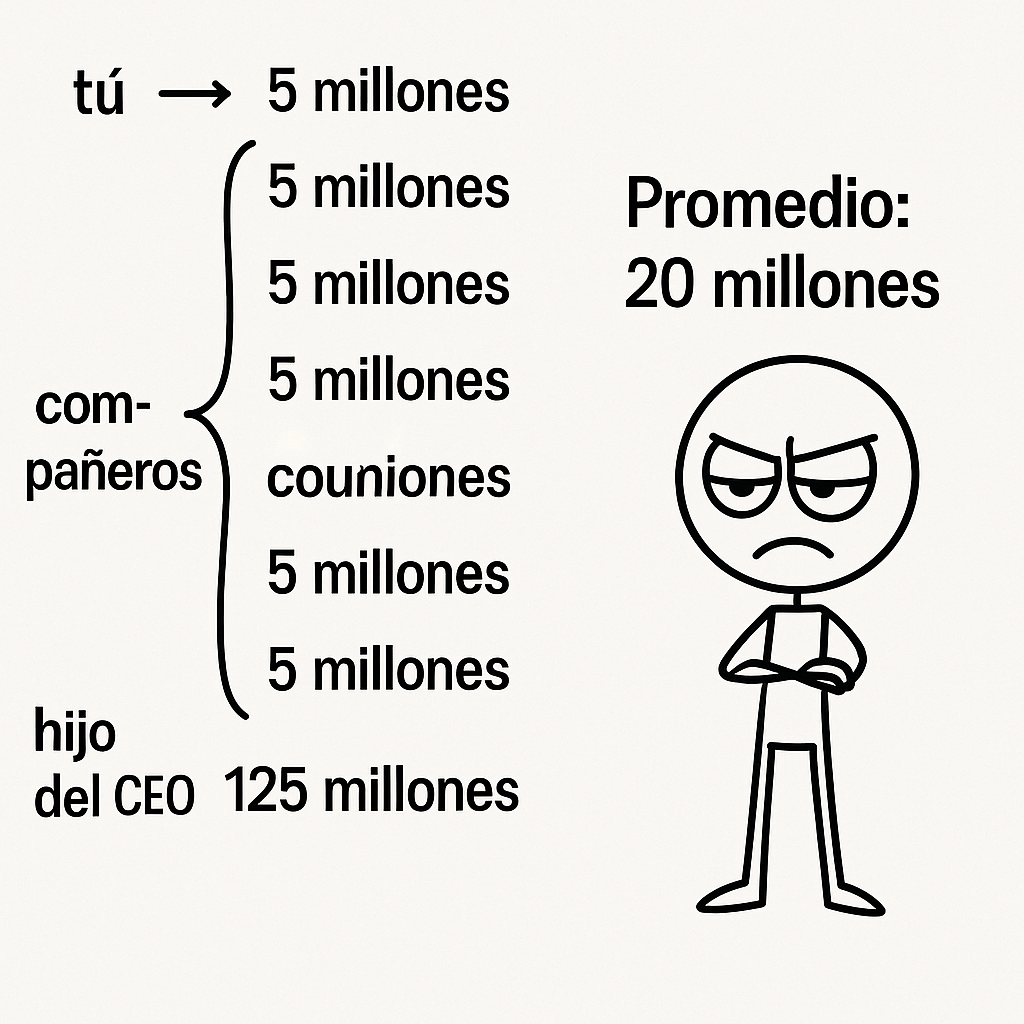
\includegraphics[width=3.64583in,height=\textheight,keepaspectratio]{img/media_2.png}
\end{center}

Aquí hay otro ejemplo donde la media es la misma en ambas situaciones
pero el contexto individual que esconde es muy diferente:

\begin{center}
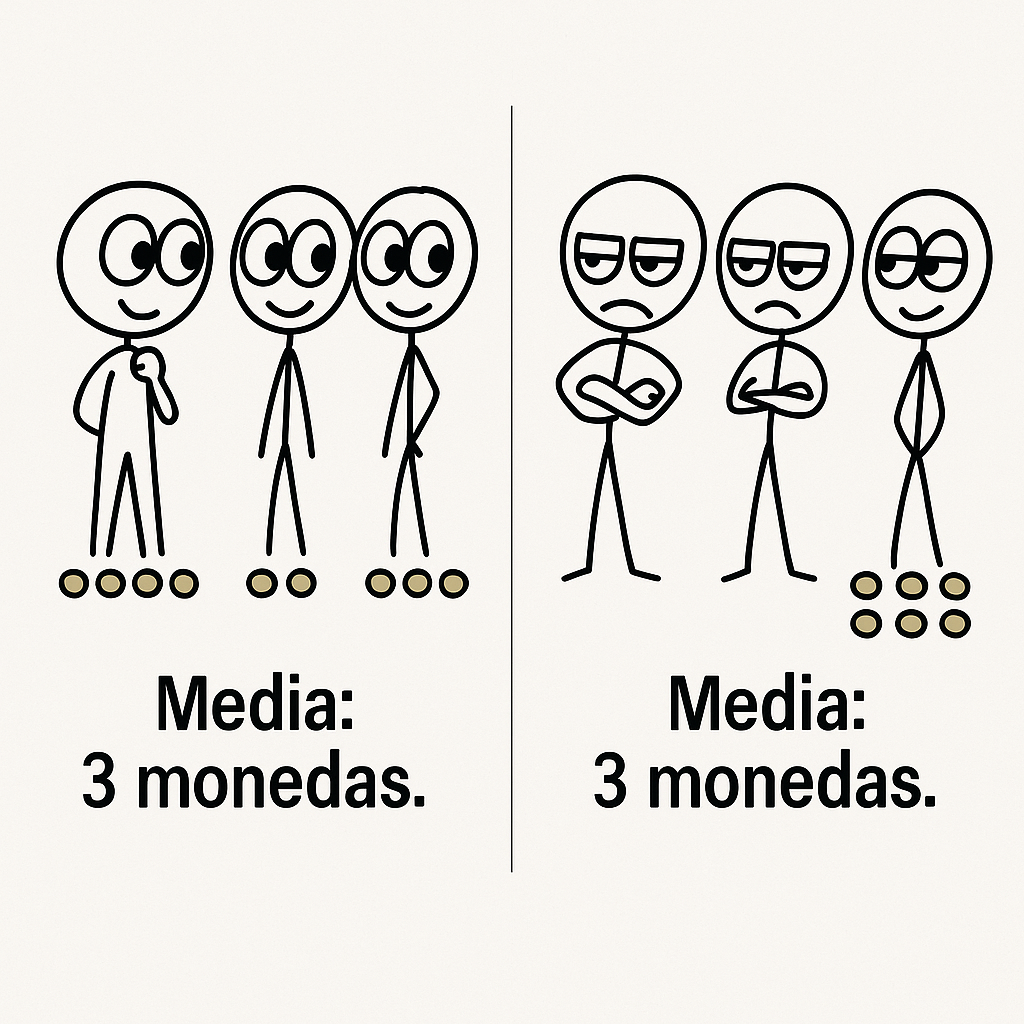
\includegraphics[width=3.64583in,height=\textheight,keepaspectratio]{img/media_3.png}
\end{center}

\subsection{Mediana}\label{mediana}

Volviendo a las calificaciones de tu restaurante, la \textbf{mediana} es
el valor que está justo en el medio cuando ordenas todas las opiniones
de menor a mayor. Esto significa que la mitad de los clientes dieron una
calificación igual o menor que la mediana, y la otra mitad dio una
calificación igual o mayor.

Por ejemplo, si tus clientes calificaron así: 3, 4, 4, 5, 5, la mediana
es 4 --- porque es el valor que divide el grupo en dos partes iguales.

\begin{tcolorbox}[enhanced jigsaw, bottomrule=.15mm, colframe=quarto-callout-tip-color-frame, breakable, colback=white, leftrule=.75mm, left=2mm, arc=.35mm, toprule=.15mm, opacityback=0, rightrule=.15mm]
\begin{minipage}[t]{5.5mm}
\textcolor{quarto-callout-tip-color}{\faLightbulb}
\end{minipage}%
\begin{minipage}[t]{\textwidth - 5.5mm}

\[
\text{Mediana} = \text{valor central en datos ordenados}
\]

\end{minipage}%
\end{tcolorbox}

Una gran ventaja de la mediana es que \textbf{no se ve afectada por
calificaciones muy bajas o muy altas} que podrían distorsionar la media.
Por ejemplo, si alguien puso un 1 o un 10, la mediana sigue mostrando el
punto medio real de la mayoría.

Sin embargo, la mediana \textbf{no nos dice qué tan dispersas están las
calificaciones a cada lado}. Por eso, para entender mejor la
variabilidad de las opiniones, necesitaremos otras medidas que veremos
más adelante.

A continuación podemos ver un ejemplo donde la mediana es usada para
entregar un mensaje erróneo:

\begin{center}
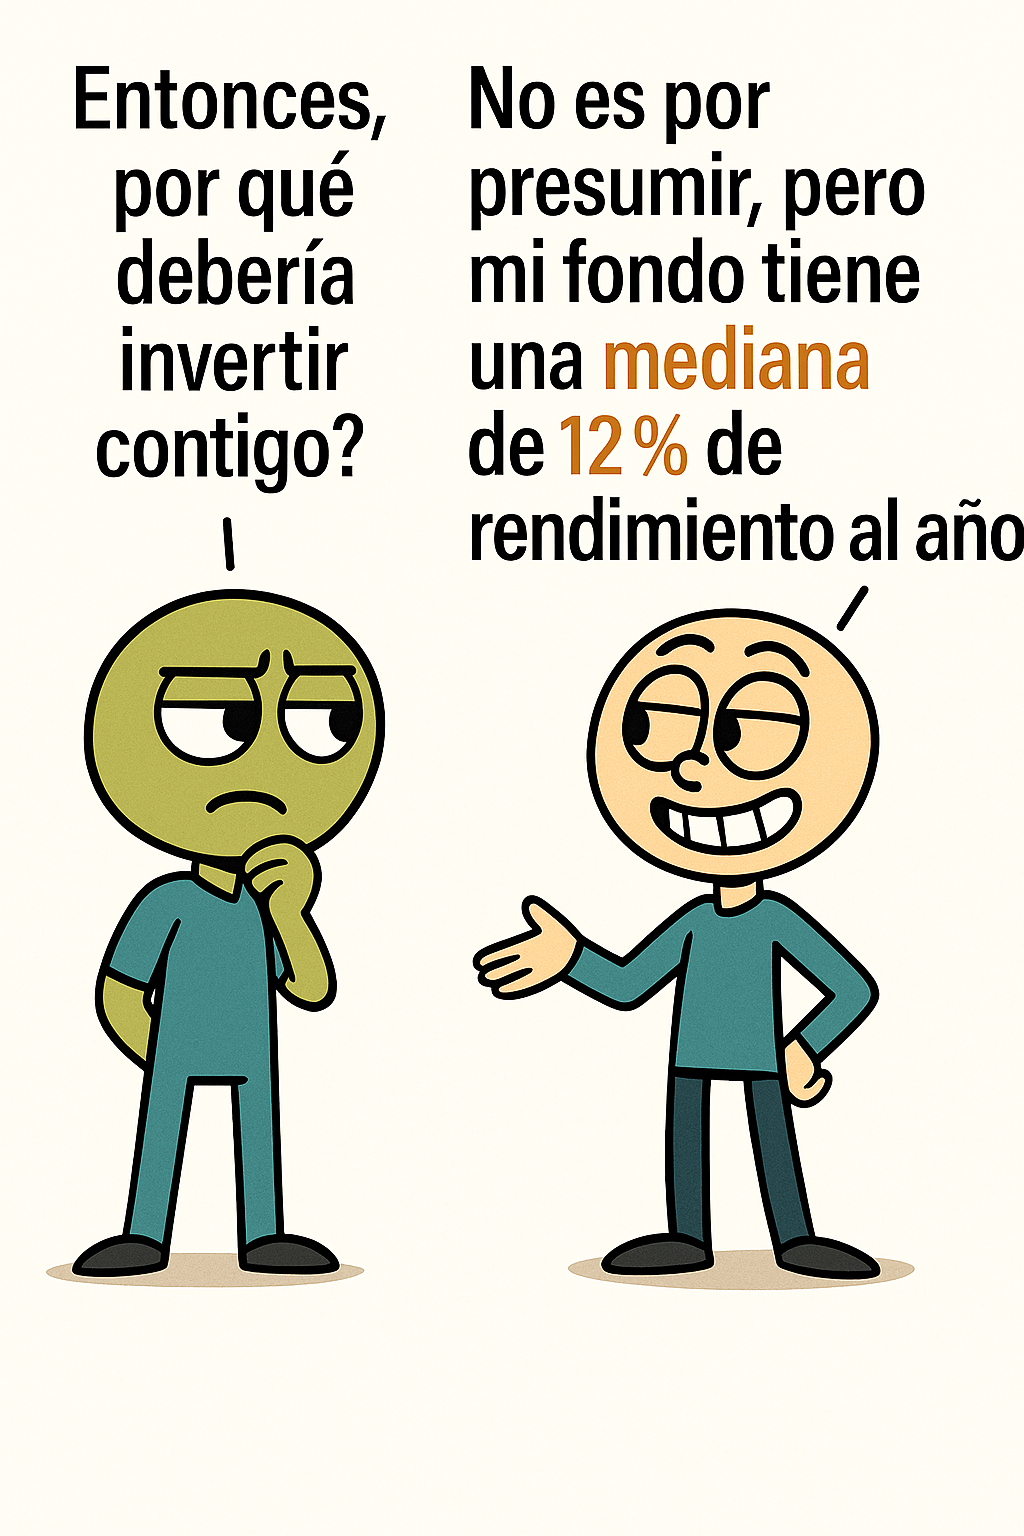
\includegraphics[width=3.64583in,height=\textheight,keepaspectratio]{img/mediana_1.png}
\end{center}

Pero, los rendimientos anuales del fondo:

\begin{center}
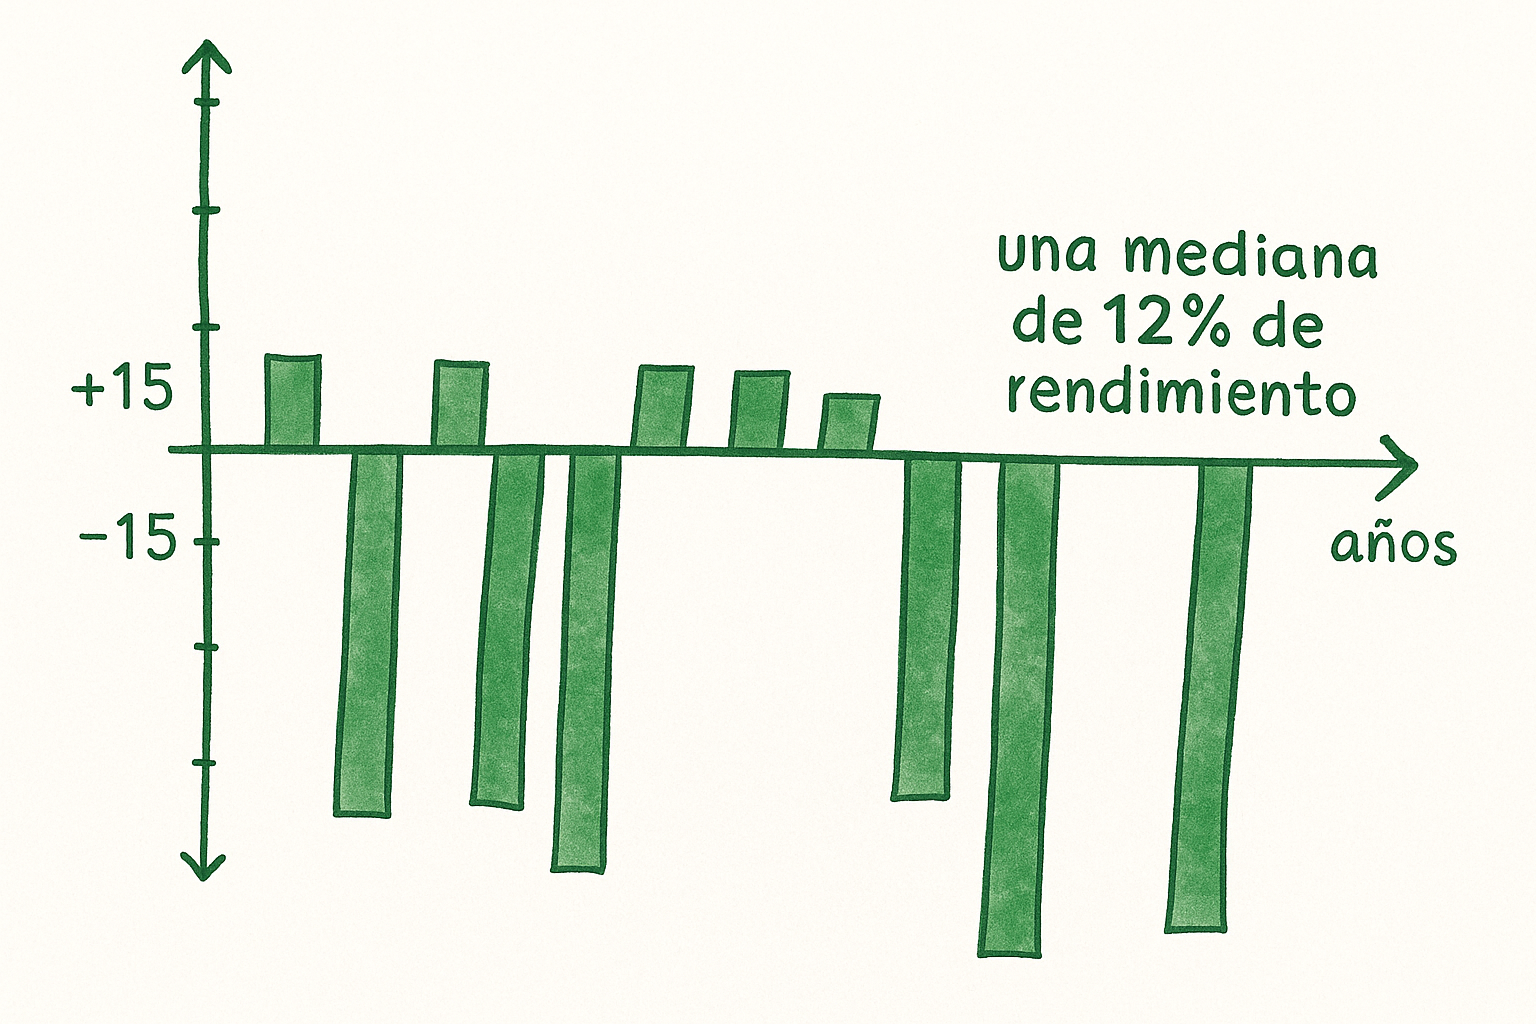
\includegraphics[width=3.64583in,height=\textheight,keepaspectratio]{img/mediana_2.png}
\end{center}

Miremos otro ejemplo donde la mediana similar no implica datos
similares. Siempre hay tener una combinación de datos para tomar
decisiones correctas

\begin{center}
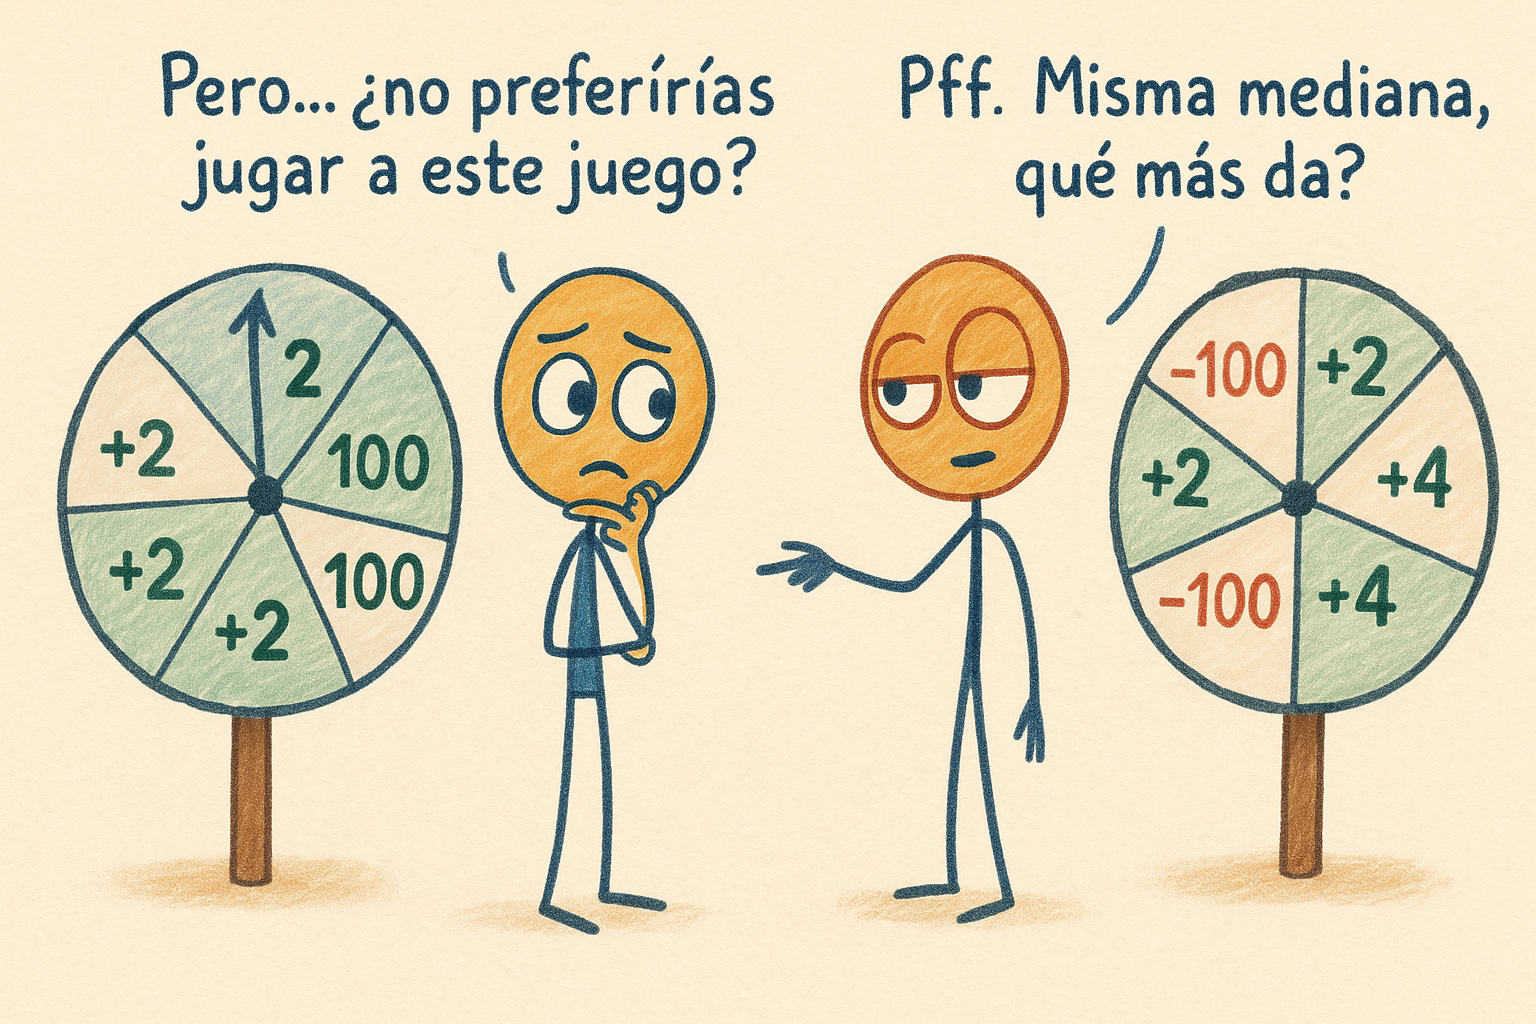
\includegraphics[width=3.64583in,height=\textheight,keepaspectratio]{img/mediana_3.png}
\end{center}

\subsection{Moda}\label{moda}

La \textbf{moda} es la calificación que más se repite entre tus
clientes. Es como la opinión más común o popular sobre tu restaurante.

Por ejemplo, si las calificaciones de tus clientes fueron: 3, 4, 4, 5,
5, tanto 4 como 5 se repiten dos veces, por lo que hay dos modas: 4 y 5.

Si no hay repeticiones exactas, se pueden agrupar en categorías y tomar
como moda la más común. Es útil especialmente con datos no numéricos,
como colores o preferencias políticas, donde no tiene sentido calcular
promedios.

\begin{tcolorbox}[enhanced jigsaw, bottomrule=.15mm, colframe=quarto-callout-tip-color-frame, breakable, colback=white, leftrule=.75mm, left=2mm, arc=.35mm, toprule=.15mm, opacityback=0, rightrule=.15mm]
\begin{minipage}[t]{5.5mm}
\textcolor{quarto-callout-tip-color}{\faLightbulb}
\end{minipage}%
\begin{minipage}[t]{\textwidth - 5.5mm}

\[
\text{Moda} = \text{valor que aparece con mayor frecuencia}
\]

\end{minipage}%
\end{tcolorbox}

Su limitación: no considera la totalidad ni la distribución de los
datos, y lo más común no siempre es lo más representativo. Miremos este
ejemplo:

\begin{center}
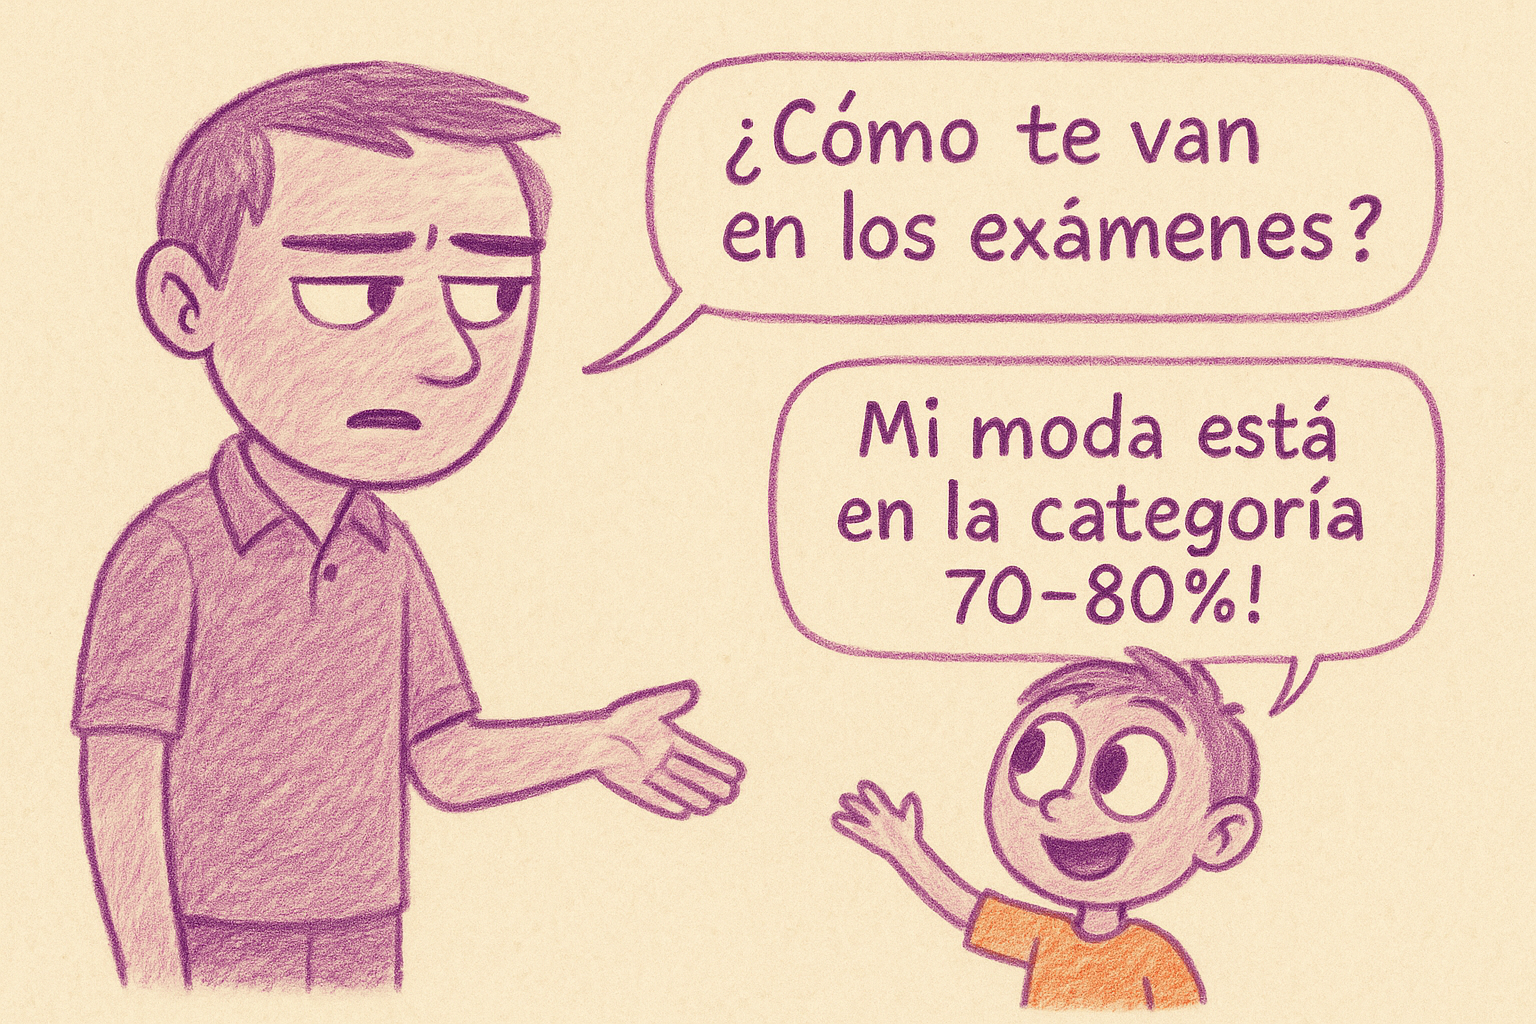
\includegraphics[width=3.64583in,height=\textheight,keepaspectratio]{img/moda_1.png}
\end{center}

\begin{center}
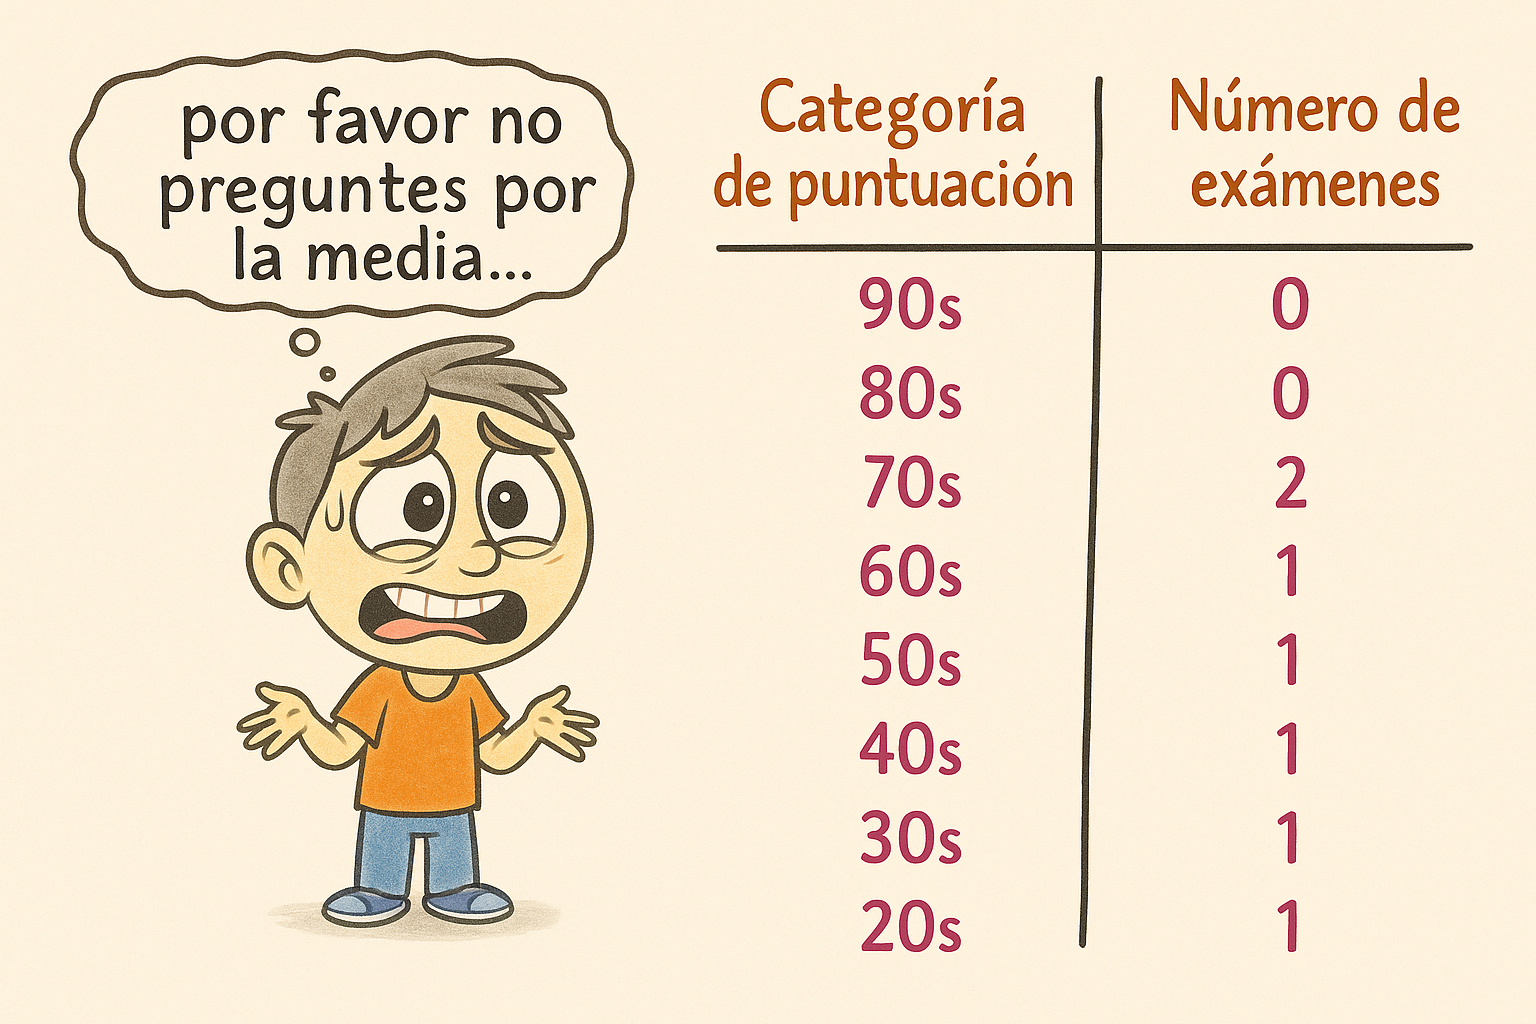
\includegraphics[width=3.64583in,height=\textheight,keepaspectratio]{img/moda_2.png}
\end{center}

\section{Medidas de Variación}\label{medidas-de-variaciuxf3n}

Las medidas de variación nos ayudan a entender qué tan diferentes o
dispersos están los datos entre sí. Es decir, nos dicen si las opiniones
o valores están muy juntos o muy separados.

\subsection{Rango}\label{rango}

Las medidas de variación nos ayudan a entender qué tan diferentes o
dispersos están los datos entre sí. Es decir, nos dicen si las opiniones
o valores están muy juntos o muy separados.

Por ejemplo, si las calificaciones en tu restaurante van desde 2 hasta
5, el rango sería:

\begin{tcolorbox}[enhanced jigsaw, bottomrule=.15mm, colframe=quarto-callout-tip-color-frame, breakable, colback=white, leftrule=.75mm, left=2mm, arc=.35mm, toprule=.15mm, opacityback=0, rightrule=.15mm]
\begin{minipage}[t]{5.5mm}
\textcolor{quarto-callout-tip-color}{\faLightbulb}
\end{minipage}%
\begin{minipage}[t]{\textwidth - 5.5mm}

\[
\text{Rango} = 5 - 2 = 3
\]

\end{minipage}%
\end{tcolorbox}

Esto nos dice que las opiniones varían en un rango de 3 puntos, desde
una calificación baja hasta una alta.

Su principal ventaja es su simplicidad, da una idea rápida del ``ancho''
del conjunto de datos.

Pero su debilidad es igual de clara, solo considera los valores
extremos, ignorando por completo todos los datos intermedios.

Miremos un ejemplo de un rango que da una impresión incorrecta:

\begin{center}
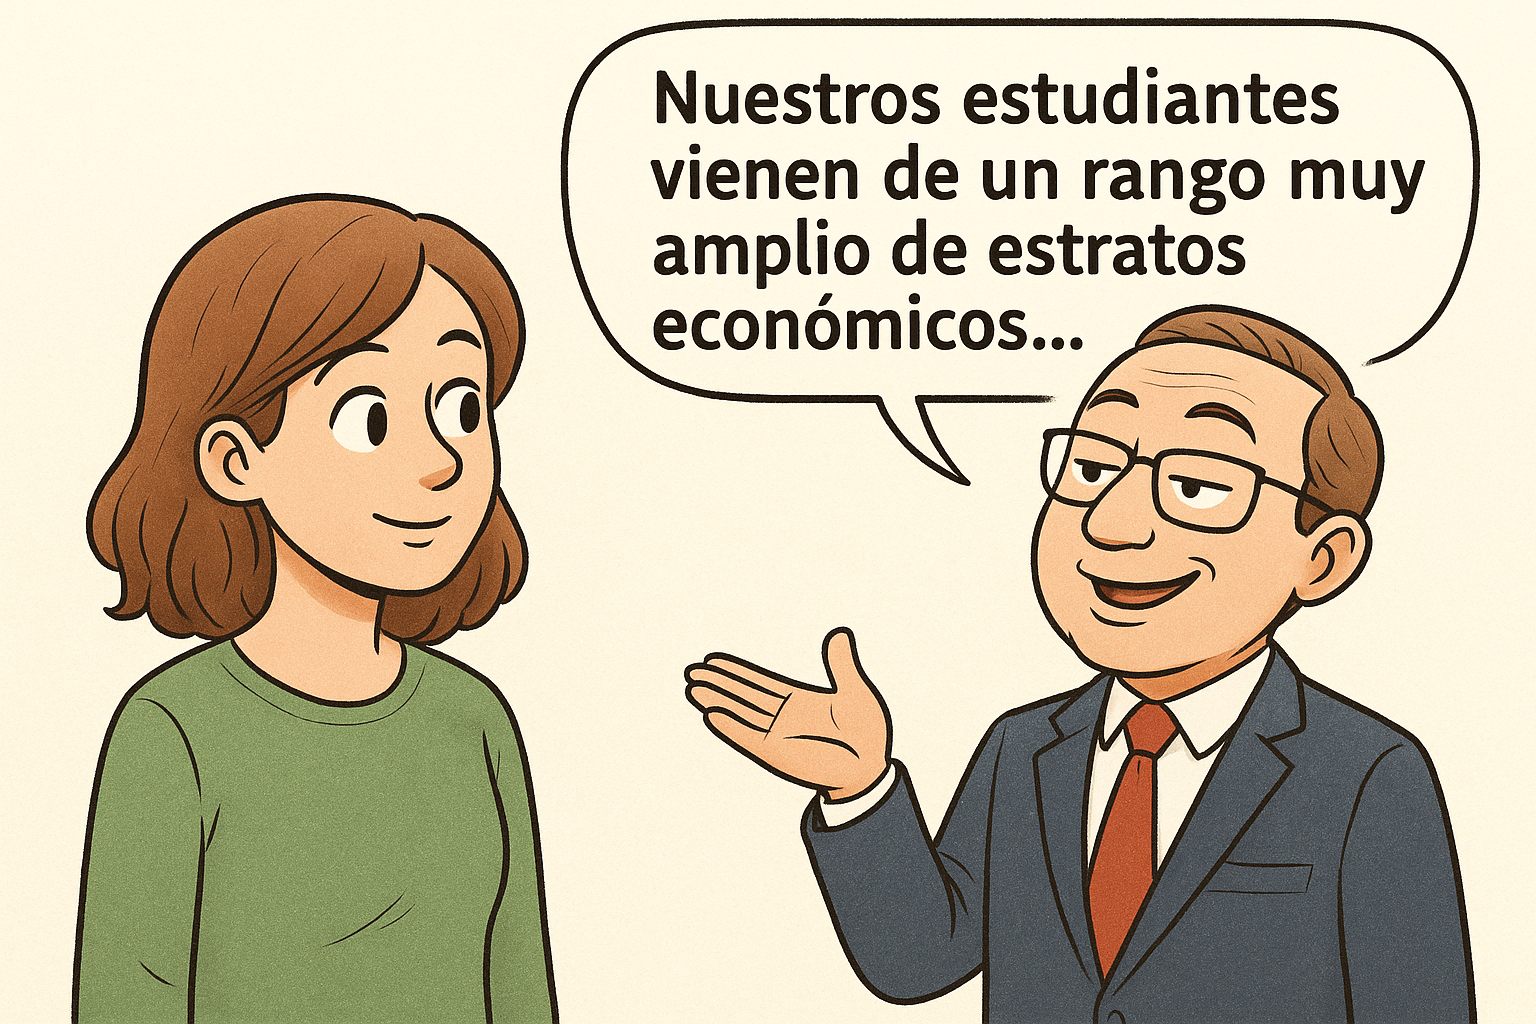
\includegraphics[width=3.64583in,height=\textheight,keepaspectratio]{img/rango_1.png}
\end{center}

\begin{center}
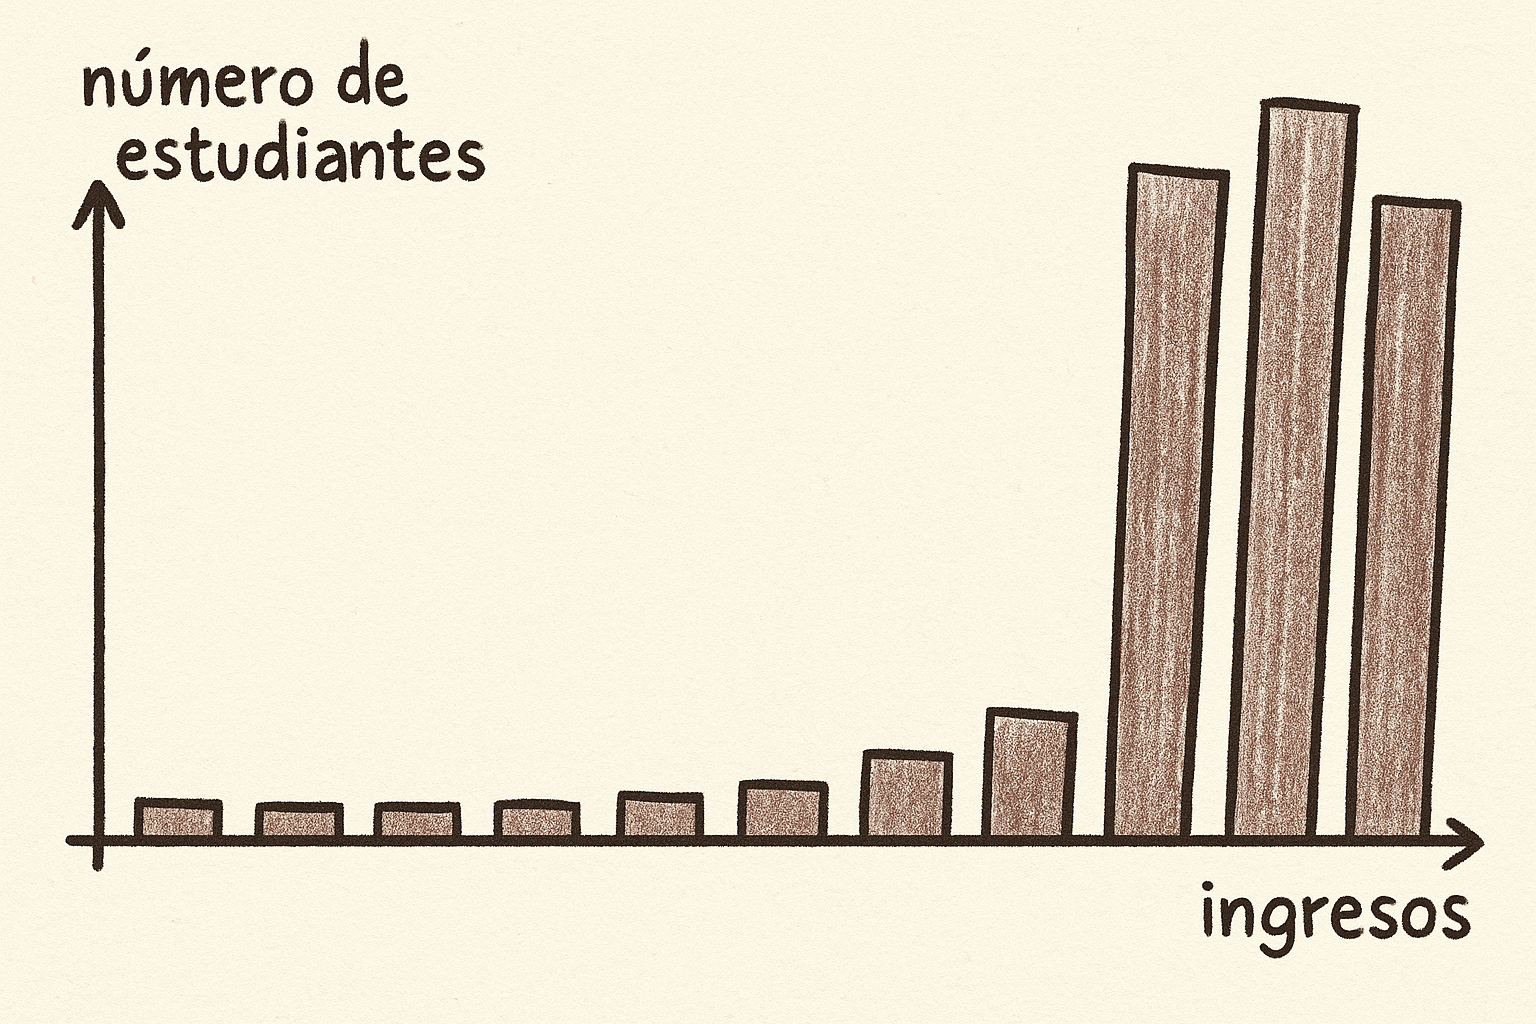
\includegraphics[width=3.64583in,height=\textheight,keepaspectratio]{img/rango_2.png}
\end{center}

\subsection{Varianza y Desviación
Estándar}\label{varianza-y-desviaciuxf3n-estuxe1ndar}

La varianza y la desviación estándar son herramientas que nos ayudan a
entender qué tan dispersos están los datos con respecto a su media.

Imagina que tienes varios números y quieres saber si están todos cerca
del promedio o si están muy separados entre sí.

Para entender qué tan dispersas están las calificaciones de tus clientes
respecto al promedio, usamos dos medidas fundamentales: la
\textbf{varianza} y la \textbf{desviación estándar}:

\begin{itemize}
\tightlist
\item
  Una desviación estándar baja significa que los datos están cerca del
  promedio.
\item
  Una alta desviación estándar indica mucha dispersión.
\end{itemize}

\begin{tcolorbox}[enhanced jigsaw, bottomrule=.15mm, colframe=quarto-callout-tip-color-frame, breakable, colback=white, leftrule=.75mm, left=2mm, arc=.35mm, toprule=.15mm, opacityback=0, rightrule=.15mm]
\begin{minipage}[t]{5.5mm}
\textcolor{quarto-callout-tip-color}{\faLightbulb}
\end{minipage}%
\begin{minipage}[t]{\textwidth - 5.5mm}

Si quisieras ``cocinar'' la varianza en tu propia cocina, la receta
sería así:

\begin{enumerate}
\def\labelenumi{\arabic{enumi}.}
\tightlist
\item
  \textbf{Encuentra la media} de todas las calificaciones.\\
\item
  \textbf{Calcula qué tan lejos está cada calificación de esa media} (la
  diferencia entre cada calificación y la media).\\
\item
  \textbf{Eleva al cuadrado cada una de esas diferencias} para evitar
  que se cancelen y para dar más peso a las diferencias grandes.\\
\item
  \textbf{Suma todas esas diferencias al cuadrado y calcula el promedio}
  dividiendo entre el número de calificaciones menos uno.
\end{enumerate}

\end{minipage}%
\end{tcolorbox}

Matemáticamente, si tienes ( n ) calificaciones ( x\_1, x\_2, \ldots,
x\_n ) y la media ( \bar\{x\} ), la varianza se calcula así:

\begin{tcolorbox}[enhanced jigsaw, bottomrule=.15mm, colframe=quarto-callout-tip-color-frame, breakable, colback=white, leftrule=.75mm, left=2mm, arc=.35mm, toprule=.15mm, opacityback=0, rightrule=.15mm]
\begin{minipage}[t]{5.5mm}
\textcolor{quarto-callout-tip-color}{\faLightbulb}
\end{minipage}%
\begin{minipage}[t]{\textwidth - 5.5mm}

\[
\text{Varianza} = s^2 = \frac{1}{n-1} \sum_{i=1}^n (x_i - \bar{x})^2
\]

\end{minipage}%
\end{tcolorbox}

Pero como la varianza está al cuadrado, no es fácil interpretarla
directamente, pues sus unidades no son las mismas que las de las
calificaciones. Por eso usamos la \textbf{desviación estándar}, que es
la raíz cuadrada de la varianza y nos da una medida en las mismas
unidades originales.

\begin{tcolorbox}[enhanced jigsaw, bottomrule=.15mm, colframe=quarto-callout-tip-color-frame, breakable, colback=white, leftrule=.75mm, left=2mm, arc=.35mm, toprule=.15mm, opacityback=0, rightrule=.15mm]
\begin{minipage}[t]{5.5mm}
\textcolor{quarto-callout-tip-color}{\faLightbulb}
\end{minipage}%
\begin{minipage}[t]{\textwidth - 5.5mm}

\[
\text{Desviación Estándar} = s = \sqrt{s^2}
\]

\end{minipage}%
\end{tcolorbox}

Por ejemplo, si las calificaciones fueron: 4, 5, 3, 4 y 5, la media es:

\begin{tcolorbox}[enhanced jigsaw, bottomrule=.15mm, colframe=quarto-callout-tip-color-frame, breakable, colback=white, leftrule=.75mm, left=2mm, arc=.35mm, toprule=.15mm, opacityback=0, rightrule=.15mm]
\begin{minipage}[t]{5.5mm}
\textcolor{quarto-callout-tip-color}{\faLightbulb}
\end{minipage}%
\begin{minipage}[t]{\textwidth - 5.5mm}

\[
\bar{x} = \frac{4 + 5 + 3 + 4 + 5}{5} = 4.2
\]

\end{minipage}%
\end{tcolorbox}

Luego, calculamos la varianza:

\begin{tcolorbox}[enhanced jigsaw, bottomrule=.15mm, colframe=quarto-callout-tip-color-frame, breakable, colback=white, leftrule=.75mm, left=2mm, arc=.35mm, toprule=.15mm, opacityback=0, rightrule=.15mm]
\begin{minipage}[t]{5.5mm}
\textcolor{quarto-callout-tip-color}{\faLightbulb}
\end{minipage}%
\begin{minipage}[t]{\textwidth - 5.5mm}

\[
s^2 = \frac{(4 - 4.2)^2 + (5 - 4.2)^2 + (3 - 4.2)^2 + (4 - 4.2)^2 + (5 - 4.2)^2}{4} = 0.7
\]

\end{minipage}%
\end{tcolorbox}

Y finalmente, la desviación estándar es:

\begin{tcolorbox}[enhanced jigsaw, bottomrule=.15mm, colframe=quarto-callout-tip-color-frame, breakable, colback=white, leftrule=.75mm, left=2mm, arc=.35mm, toprule=.15mm, opacityback=0, rightrule=.15mm]
\begin{minipage}[t]{5.5mm}
\textcolor{quarto-callout-tip-color}{\faLightbulb}
\end{minipage}%
\begin{minipage}[t]{\textwidth - 5.5mm}

\[
s = \sqrt{0.7} \approx 0.84
\]

\end{minipage}%
\end{tcolorbox}

Esto significa que, en promedio, las calificaciones se alejan de la
media en aproximadamente 0.84 puntos.

A diferencia del rango, que solo considera los valores más extremos, la
varianza y la desviación estándar toman en cuenta todos los datos. Por
eso ofrecen una visión más completa de la dispersión. Sin embargo,
también tienen una desventaja: si hay un solo valor muy alejado (un
valor extremo), puede aumentar mucho la varianza, aunque la mayoría de
los datos estén cerca de la media. Mira el ejemplo a continuación, para
entenderlo mejor:

\begin{center}
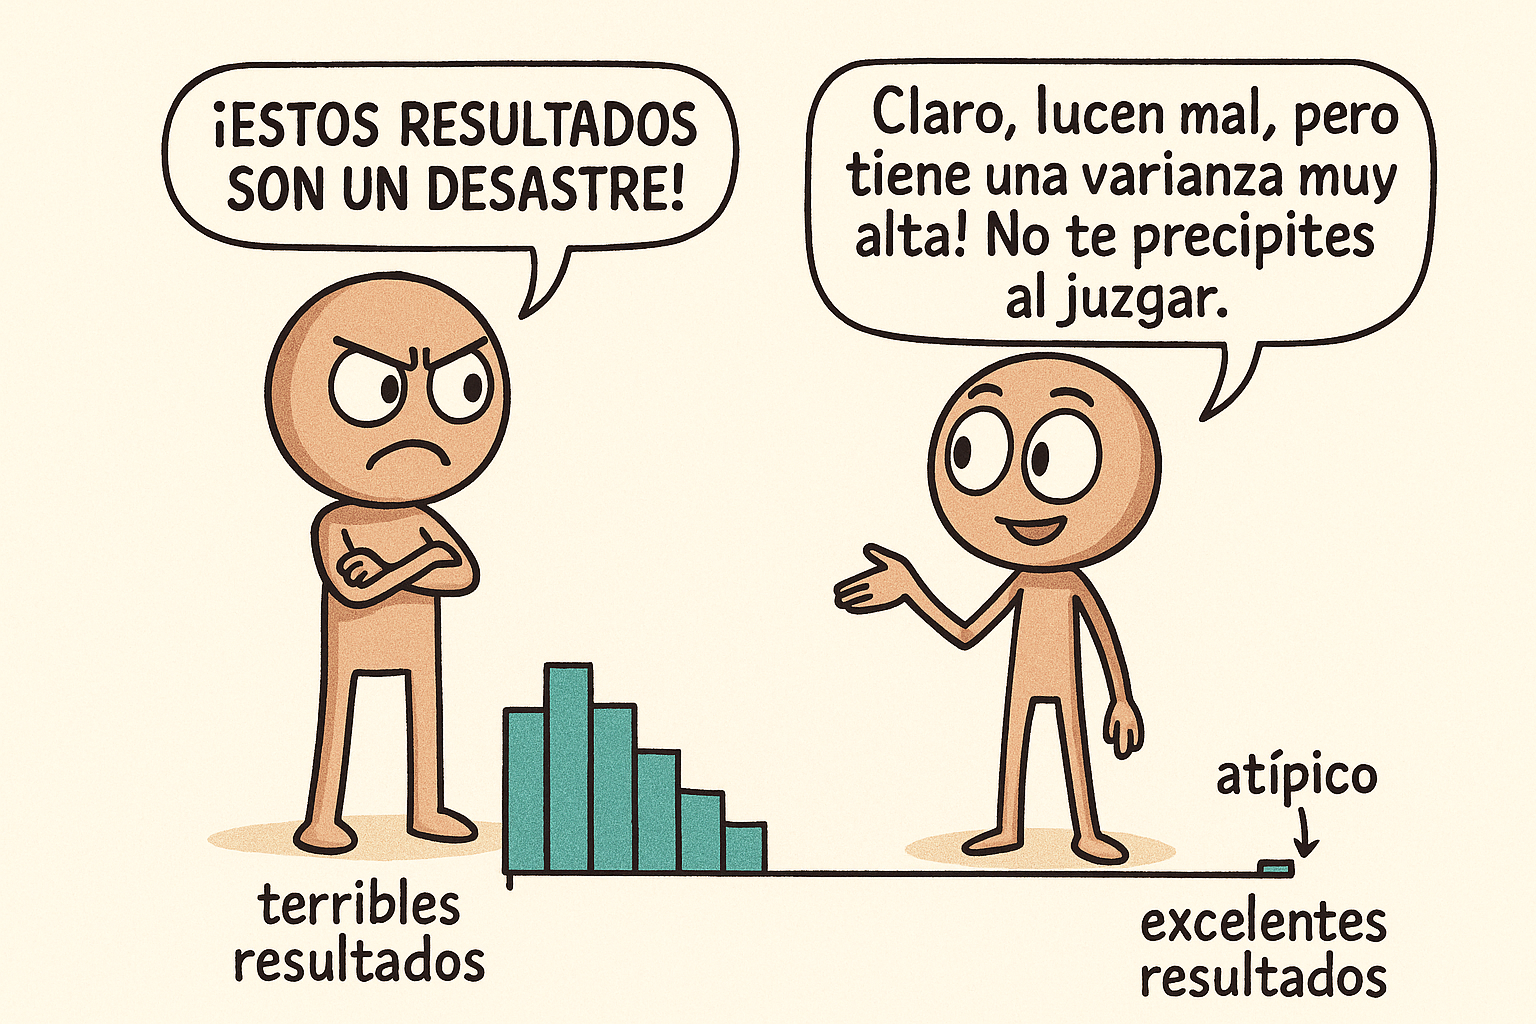
\includegraphics[width=3.64583in,height=\textheight,keepaspectratio]{img/varianza_1.png}
\end{center}

\subsection{Percentil, Cuartiles}\label{percentil-cuartiles}

Imagina que quieres saber cómo se comparan las calificaciones de tus
clientes con todas las demás. Los \textbf{percentiles} nos ayudan a
entender la posición relativa de una calificación dentro del grupo.

Un percentil nos dice qué porcentaje de las calificaciones está por
debajo de cierto valor. Por ejemplo, el \textbf{percentil 25} indica el
punto bajo el cual se encuentra el 25\% de las calificaciones más bajas.

Si una calificación está en el percentil 25, significa que el 25\% de
los clientes dio una calificación igual o menor que esa, y el 75\% dio
una calificación más alta.

Esto es útil para entender la posición relativa de una calificación sin
que las opiniones muy bajas o muy altas influyan demasiado.

Sin embargo, los percentiles \textbf{no nos dicen qué tan separados
están los datos ni qué tan extremos son esos valores.}

Los \textbf{cuartiles} son un tipo especial de percentiles que dividen
las calificaciones en cuatro grupos iguales, cada uno con el 25\% de las
opiniones.

\begin{itemize}
\tightlist
\item
  El \textbf{primer cuartil (Q1)} es igual al percentil 25.\\
\item
  El \textbf{segundo cuartil (Q2)} es la mediana, el punto medio
  (percentil 50).\\
\item
  El \textbf{tercer cuartil (Q3)} es el percentil 75.
\end{itemize}

Esto permite resumir cómo se distribuyen las calificaciones y saber en
qué grupo se ubica cada opinión, incluso si hay calificaciones muy bajas
o muy altas.

\subsection{Rango Intercuartílico
(RIC)}\label{rango-intercuartuxedlico-ric}

Para entender mejor cómo varían las calificaciones en la parte central
de los datos, usamos el \textbf{Rango Intercuartílico}, o \textbf{RIC},
que es la diferencia entre el tercer cuartil y el primer cuartil:

\begin{tcolorbox}[enhanced jigsaw, bottomrule=.15mm, colframe=quarto-callout-tip-color-frame, breakable, colback=white, leftrule=.75mm, left=2mm, arc=.35mm, toprule=.15mm, opacityback=0, rightrule=.15mm]
\begin{minipage}[t]{5.5mm}
\textcolor{quarto-callout-tip-color}{\faLightbulb}
\end{minipage}%
\begin{minipage}[t]{\textwidth - 5.5mm}

\[
RIC = Q3 - Q1
\]

\end{minipage}%
\end{tcolorbox}

El RIC mide la dispersión del 50\% central de las calificaciones,
ignorando las opiniones más bajas y más altas que podrían ser atípicas.

Por ejemplo, si el primer cuartil es 3.5 y el tercer cuartil es 4.5, el
RIC sería:

\begin{tcolorbox}[enhanced jigsaw, bottomrule=.15mm, colframe=quarto-callout-tip-color-frame, breakable, colback=white, leftrule=.75mm, left=2mm, arc=.35mm, toprule=.15mm, opacityback=0, rightrule=.15mm]
\begin{minipage}[t]{5.5mm}
\textcolor{quarto-callout-tip-color}{\faLightbulb}
\end{minipage}%
\begin{minipage}[t]{\textwidth - 5.5mm}

\[
RIC = 4.5 - 3.5 = 1.0
\]

\end{minipage}%
\end{tcolorbox}

Esto indica que la mitad central de las calificaciones está dentro de un
rango de 1 punto, mostrando cuán consistentes son las opiniones
principales.

El RIC es muy útil porque, a diferencia del rango total, \textbf{no se
ve afectado por calificaciones extremas} y nos da una idea clara de la
variabilidad donde está la mayoría de los datos.

\subsection{Diagrama de Caja y Brazos
(Boxplot)}\label{diagrama-de-caja-y-brazos-boxplot}

Para visualizar fácilmente la distribución de las calificaciones de tus
clientes, usamos el \textbf{diagrama de caja y brazos}, también conocido
como \textbf{boxplot}.

Este gráfico muestra en una caja la parte central de los datos, desde el
primer cuartil (Q1) hasta el tercer cuartil (Q3), con una línea en la
mediana (Q2).

Además, los ``brazos'' o líneas que salen de la caja se extienden hasta
los valores mínimos y máximos dentro de un rango razonable, ayudándonos
a identificar si hay calificaciones atípicas o muy extremas.

Así, con un solo gráfico puedes ver:

\begin{itemize}
\tightlist
\item
  Dónde está la mayoría de las calificaciones (la caja).\\
\item
  La calificación típica (la mediana dentro de la caja).\\
\item
  La dispersión general (la longitud de la caja y brazos).\\
\item
  Valores extremos o posibles opiniones fuera de lo común (puntos fuera
  de los brazos).
\end{itemize}

El diagrama de caja es una herramienta poderosa para resumir y comparar
la distribución de las calificaciones de forma rápida y visual.

Este sería un ejemplo en R:

\begin{Shaded}
\begin{Highlighting}[]
\CommentTok{\# Instalar paquetes si no están instalados}
\CommentTok{\# install.packages(c("ggplot2", "ggthemes", "viridis"))}

\FunctionTok{library}\NormalTok{(ggplot2)}
\FunctionTok{library}\NormalTok{(ggthemes)}
\end{Highlighting}
\end{Shaded}

\begin{verbatim}
Warning: package 'ggthemes' was built under R version 4.3.3
\end{verbatim}

\begin{Shaded}
\begin{Highlighting}[]
\FunctionTok{library}\NormalTok{(viridis)}
\end{Highlighting}
\end{Shaded}

\begin{verbatim}
Warning: package 'viridis' was built under R version 4.3.3
\end{verbatim}

\begin{verbatim}
Loading required package: viridisLite
\end{verbatim}

\begin{Shaded}
\begin{Highlighting}[]
\CommentTok{\# Crear datos simulados de calificaciones para 3 restaurantes}
\FunctionTok{set.seed}\NormalTok{(}\DecValTok{123}\NormalTok{)}

\NormalTok{datos }\OtherTok{\textless{}{-}} \FunctionTok{data.frame}\NormalTok{(}
  \AttributeTok{restaurante =} \FunctionTok{rep}\NormalTok{(}\FunctionTok{c}\NormalTok{(}\StringTok{"Mi Restaurante"}\NormalTok{, }\StringTok{"Competidor 1"}\NormalTok{, }\StringTok{"Competidor 2"}\NormalTok{), }\AttributeTok{each =} \DecValTok{50}\NormalTok{),}
  \AttributeTok{calificacion =} \FunctionTok{c}\NormalTok{(}
    \FunctionTok{rnorm}\NormalTok{(}\DecValTok{50}\NormalTok{, }\AttributeTok{mean =} \DecValTok{4}\NormalTok{, }\AttributeTok{sd =} \FloatTok{0.7}\NormalTok{),  }\CommentTok{\# Mi restaurante: variación media}
    \FunctionTok{rnorm}\NormalTok{(}\DecValTok{50}\NormalTok{, }\AttributeTok{mean =} \FloatTok{3.5}\NormalTok{, }\AttributeTok{sd =} \FloatTok{1.2}\NormalTok{), }\CommentTok{\# Competidor 1: más variación (peor control)}
    \FunctionTok{rnorm}\NormalTok{(}\DecValTok{50}\NormalTok{, }\AttributeTok{mean =} \FloatTok{4.2}\NormalTok{, }\AttributeTok{sd =} \FloatTok{0.3}\NormalTok{)  }\CommentTok{\# Competidor 2: poca variación (muy consistente)}
\NormalTok{  )}
\NormalTok{)}

\CommentTok{\# Limitar calificaciones entre 1 y 5}
\NormalTok{datos}\SpecialCharTok{$}\NormalTok{calificacion }\OtherTok{\textless{}{-}} \FunctionTok{pmin}\NormalTok{(}\FunctionTok{pmax}\NormalTok{(datos}\SpecialCharTok{$}\NormalTok{calificacion, }\DecValTok{1}\NormalTok{), }\DecValTok{5}\NormalTok{)}

\CommentTok{\# Boxplot comparativo con viridis y theme\_few}
\FunctionTok{ggplot}\NormalTok{(datos, }\FunctionTok{aes}\NormalTok{(}\AttributeTok{x =}\NormalTok{ restaurante, }\AttributeTok{y =}\NormalTok{ calificacion, }\AttributeTok{fill =}\NormalTok{ restaurante)) }\SpecialCharTok{+}
  \FunctionTok{geom\_boxplot}\NormalTok{(}\AttributeTok{outlier.shape =} \DecValTok{16}\NormalTok{, }\AttributeTok{outlier.size =} \DecValTok{2}\NormalTok{, }\AttributeTok{alpha =} \FloatTok{0.8}\NormalTok{) }\SpecialCharTok{+}
  \FunctionTok{scale\_fill\_viridis}\NormalTok{(}\AttributeTok{discrete =} \ConstantTok{TRUE}\NormalTok{, }\AttributeTok{option =} \StringTok{"D"}\NormalTok{) }\SpecialCharTok{+}
  \FunctionTok{labs}\NormalTok{(}
    \AttributeTok{title =} \StringTok{"Comparación de Calificaciones entre Restaurantes"}\NormalTok{,}
    \AttributeTok{x =} \StringTok{"Restaurante"}\NormalTok{,}
    \AttributeTok{y =} \StringTok{"Calificación (1 a 5)"}
\NormalTok{  ) }\SpecialCharTok{+}
  \FunctionTok{theme\_few}\NormalTok{() }\SpecialCharTok{+}
  \FunctionTok{theme}\NormalTok{(}
    \AttributeTok{legend.position =} \StringTok{"none"}\NormalTok{,}
    \AttributeTok{plot.title =} \FunctionTok{element\_text}\NormalTok{(}\AttributeTok{hjust =} \FloatTok{0.5}\NormalTok{, }\AttributeTok{size =} \DecValTok{16}\NormalTok{, }\AttributeTok{face =} \StringTok{"bold"}\NormalTok{)}
\NormalTok{  )}
\end{Highlighting}
\end{Shaded}

\begin{center}
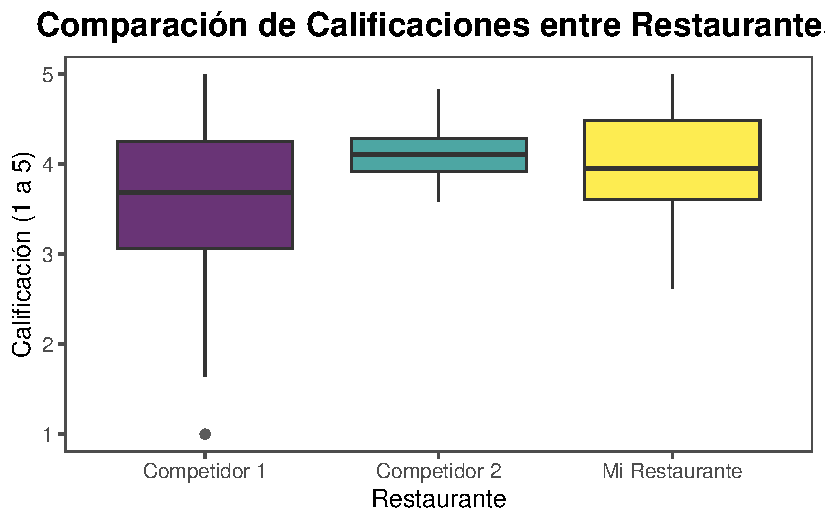
\includegraphics[width=3.64583in,height=\textheight,keepaspectratio]{capitulo3_files/figure-pdf/unnamed-chunk-12-1.pdf}
\end{center}

\section{Medidas de Relación
Lineal}\label{medidas-de-relaciuxf3n-lineal}

Estas nos dicen si dos variables están relacionadas entre sí.

Imagina que además de las calificaciones que dan tus clientes, también
registras cuántas veces visitan tu restaurante al mes. Quieres entender
si estas dos cosas están relacionadas: ¿los clientes que visitan más
tienden a dar mejores calificaciones? ¿O tal vez ocurre lo contrario?

\subsection{Covarianza}\label{covarianza}

La \textbf{covarianza} es una medida que nos indica si dos variables
tienden a subir o bajar juntas.

\begin{itemize}
\tightlist
\item
  Si la covarianza es \textbf{positiva}, significa que cuando una
  variable aumenta, la otra también tiende a aumentar.\\
\item
  Si es \textbf{negativa}, cuando una variable sube, la otra tiende a
  bajar.\\
\item
  Si es cercana a \textbf{cero}, no hay una relación lineal clara entre
  ellas.
\end{itemize}

Sin embargo, la covarianza solo nos dice la dirección de la relación,
pero no qué tan fuerte es, y su valor depende de las unidades de las
variables, lo que dificulta compararla entre diferentes pares de
variables. Es decir, no puedo comparar dos covarianzas de dos variables
distintas.

\subsection{Coeficiente de
Correlación}\label{coeficiente-de-correlaciuxf3n}

Para solucionar esas limitaciones, usamos el \textbf{coeficiente de
correlación}.

Este coeficiente es una versión estandarizada de la covarianza que
siempre toma un valor entre -1 y 1:

\begin{itemize}
\tightlist
\item
  \textbf{1} indica una relación lineal positiva perfecta: a más
  visitas, mejores calificaciones, siempre.\\
\item
  \textbf{-1} indica una relación lineal negativa perfecta: a más
  visitas, peores calificaciones, siempre.\\
\item
  \textbf{0} indica que no hay una relación lineal significativa entre
  las variables.
\end{itemize}

Por ejemplo, un coeficiente de correlación de 0.7 entre visitas y
calificaciones indica una relación positiva fuerte: los clientes que
visitan más suelen estar más satisfechos.

Sin embargo, que haya correlación no implica que una variable
\textbf{cause} la otra, sólo que existe alguna relación la cual incluso
puede ser casualidad no causalidad. Miremos un ejemplo donde correlación
no implica causalidad:

\begin{center}

\includegraphics[width=3.64583in,height=\textheight,keepaspectratio]{img/correlacion_1.png}
\end{center}

\begin{center}
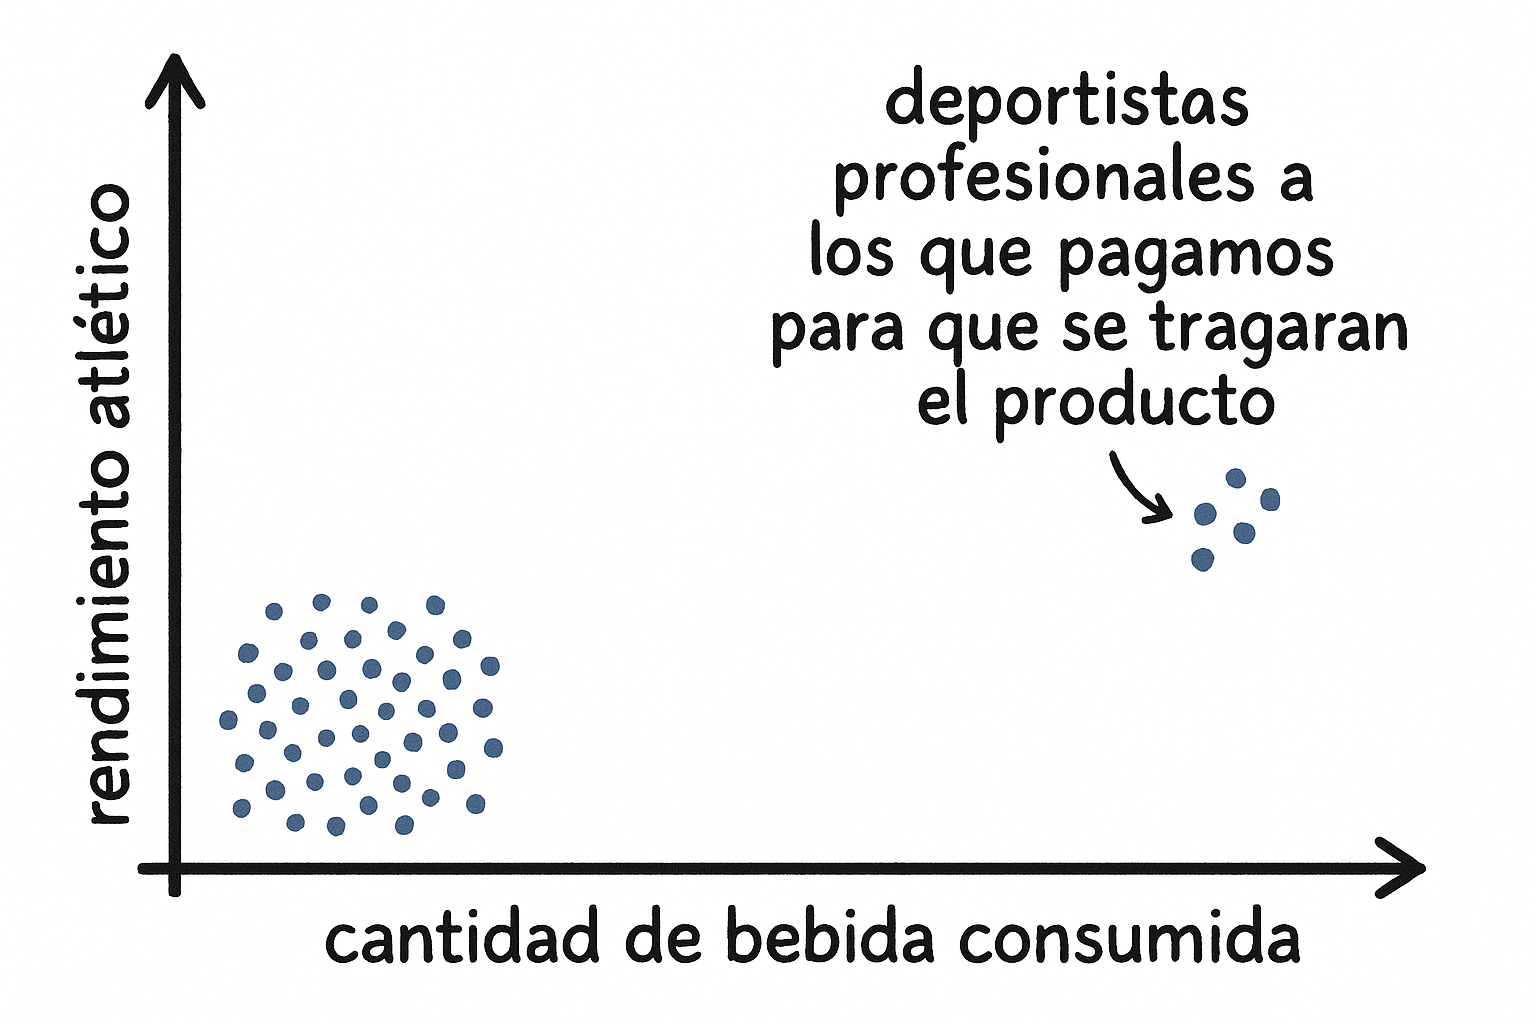
\includegraphics[width=3.64583in,height=\textheight,keepaspectratio]{img/correlacion_2.png}
\end{center}

\bookmarksetup{startatroot}

\chapter{Contando Historias Claras con
Gráficos}\label{contando-historias-claras-con-gruxe1ficos}

Imagina que entras a una librería y tomas un libro por curiosidad. Lo
abres en una página al azar y notas que algo llama inmediatamente tu
atención: un gráfico con colores vibrantes, líneas claras y un mensaje
sencillo de entender. ¿Qué hizo que te fijaras primero en ese gráfico?
Vamos a descubrirlo.

\section{¿Qué es una buena
gráfica?}\label{quuxe9-es-una-buena-gruxe1fica}

Una gráfica efectiva no solo muestra números o barras. Es una
herramienta poderosa que cuenta historias, explica conceptos y revela
información de manera clara y sencilla. Algunas claves importantes para
una buena gráfica son:

\begin{itemize}
\tightlist
\item
  \textbf{Claridad en la rotulación:} Todos los elementos del gráfico
  deben estar claramente identificados.
\item
  \textbf{Sin ornamentación innecesaria:} Menos es más. No necesitas
  adornos que distraigan del mensaje principal.
\item
  \textbf{Uso juicioso del color:} Elige colores que ayuden a resaltar
  lo más importante.
\item
  \textbf{Una historia simple y clara:} El gráfico debe ser fácil de
  entender a simple vista.
\end{itemize}

\section{Cómo leemos gráficos: principios
clave}\label{cuxf3mo-leemos-gruxe1ficos-principios-clave}

Existen cinco principios que describen cómo observamos y entendemos las
gráficas:

\begin{enumerate}
\def\labelenumi{\arabic{enumi}.}
\tightlist
\item
  \textbf{No vamos en orden:} Nuestra vista puede empezar por cualquier
  parte del gráfico. Es posible que no leas el título hasta mucho
  después.
\item
  \textbf{Primero vemos lo que se destaca:} Automáticamente nuestros
  ojos buscan picos, colores intensos, intersecciones o valores
  atípicos.
\item
  \textbf{Vemos solo unas pocas cosas a la vez:} Demasiada información
  puede confundir. Concéntrate en pocos puntos clave.
\item
  \textbf{Buscamos significado y conexiones:} Al ver algo llamativo,
  inmediatamente intentamos entender qué significa.
\item
  \textbf{Nos basamos en convenciones y metáforas:} Interpretamos
  gráficos usando lo que ya conocemos y lo que hemos aprendido antes.
\end{enumerate}

\section{El uso inteligente del
color}\label{el-uso-inteligente-del-color}

Supongamos que quieres mostrar cómo han evolucionado las ventas de
productos electrónicos en una tienda durante el último año. Tienes
información de varias categorías como televisores, teléfonos y
audífonos. ¿Cómo resaltas lo más importante?

\begin{itemize}
\item
  Primero, piensa cuál es la pregunta más importante que debería
  responder tu gráfico. ¿Quizás mostrar que los teléfonos han superado
  ampliamente las ventas de los otros productos?
\item
  Usa un color vibrante como el azul intenso para la categoría principal
  (teléfonos) y usa tonos grises o menos saturados para el resto
  (televisores y audífonos). El contraste inmediatamente enfocará la
  atención hacia los teléfonos, destacando claramente tu punto.
\end{itemize}

\textbf{Consejo práctico:} Haz todo gris excepto lo más importante. El
gris es tu aliado, resaltando por contraste el mensaje central del
gráfico.

\section{Conclusión}\label{conclusiuxf3n}

La próxima vez que diseñes un gráfico, recuerda que estás contando una
historia. Decide qué quieres destacar, usa colores sabiamente y mantén
la claridad y simplicidad. Así, tus lectores no solo verán un gráfico,
sino que comprenderán y recordarán tu mensaje.

\bookmarksetup{startatroot}

\chapter{}\label{section}




\end{document}
